% include the figures path relative to the master file \graphicspath{
{./content/method/figures/} } \section{Background}\label{sec:review} This
section reviews works straightly addressing the problem of classifying
\gls{oct} volumes as normal or abnormal, regardless of the target pathology.
The methods are categorized in terms of its learning strategy, namely:
supervised or semi-supervised.



Venhuizen\,\textit{et al.} proposed a method for \gls{oct} images
classification using the \gls{bow} models~\cite{Venhuizen2015}.  The method
starts with the detection and selection of keypoints in each individual
B-scan, by keeping the most salient points corresponding to the top $3 \%$
of the vertical gradient values. Then, a texton of size $9 \times 9$ pixels
is extracted around each keypoint, and \gls{pca} is applied to reduce the
dimension of every texton to get a feature vector of size $9$.  All
extracted feature vectors are used to create a codebook using
\textit{k}-means clustering.  Then, each \gls{oct} volume is represented in
terms of this codebook and is characterized as a histogram that captures
the codebook occurrences.  These histograms are used as feature vector to
train a \gls{rf} with a maximum of $100$ trees.  The method was used to
classify \gls{oct} volumes between \gls{amd} and normal cases and achieved
an \gls{auc} of $0.984$ with a dataset of $384$ \gls{oct} volumes.

Srinivasan\,\textit{et~al.}~\cite{Srinivasan2014} proposed a classification
method to distinguish \gls{dme}, \gls{amd} and normal \gls{sdoct} volumes.
The \gls{oct} images are pre-processed by reducing the speckle noise by
enhancing the sparsity in a transform-domain and flattening the retinal
curvature to reduce the inter-patient variations.  Then, \gls{hog} are
extracted for each slice of a volume and a linear \gls{svm} is used for
classification.  On a dataset of 45 patients equally subdivided into the
three aforementioned classes, this method leads to a correct classification
rate of $100 \%$, $100 \%$ and $86.67 \%$ for normal, \gls{dme} and
\gls{amd} patients, respectively.  The images that have been used in their
paper, are publicly available but are already preprocessed (i.e.,
denoised), have different sizes for the \gls{oct} volumes, do not offer a
huge variability in term of \gls{dme} lesions, and some of them, without
specifying which, have been excluded for the training phase; all these
reasons prevent us from using this dataset to benchmark our work.


Liu\,\textit{et al.} proposed a methodology for detecting macular pathology
in \gls{oct} images using \gls{lbp} and gradient information as
attributes~\cite{Liu2011}.  The method starts by aligning and flattening the
images and creating a $3$-level multi-scale spatial pyramid.  The edge and
\gls{lbp} histograms are then extracted from each block of every level of
the pyramid.  %is created and edge and \gls{lbp} histograms are extracted in
each block at every level of the pyramid.  All the obtained histograms are
concatenated into a global descriptor whose dimensions are reduced using
\gls{pca}.  Finally a \gls{svm} with an \gls{rbf} kernel is used as
classifier.  The method achieved good results in detection \gls{oct} scan
containing different pathology such as \gls{dme} or \gls{amd}, with an
\gls{auc} of $0.93$ using a dataset of $326$ \gls{oct} scans.


The proposed method by Lemaitre~\emph{et~al.}~\cite{Lemaintre2015miccaiOCT} is
based on \gls{lbp} features to describe the texture of \gls{oct} images and
dictionary learning using the \gls{bow} models~\cite{Sivic2003}.  Our later
study proposes a standard classification procedure to differentiate between
\gls{dme} and normal \gls{sdoct} volumes~\cite{Lemaitre2015}The data is
pre-processed using \gls{nlm} filtering.  The volumes are mapped into discrete
set of structures namely: local, when these structures correspond to patches;
or global, when the structures correspond to volume slices or the whole
volume.  These structures are described in terms of texture using \gls{lbp} or
\gls{lbptop} and encoded using histogram, \gls{pca} or \gls{bow} to produce a
single feature vector in order to present the volumes to a \gls{rf}
classifeir.  This methodology was tested against Venhuizen\,\textit{et
al.}~\cite{Venhuizen2015} using public and non-public datasets showing an
improvement within the results achieving a \gls{se} of 87.5\% and a \gls{sp}
of 75\%.



% \begin{landscape}
\begin{table}
\caption{Summary of the state-of-the-art methods.}
\resizebox{1.05\linewidth}{!}{
\scriptsize{
\begin{tabular}{l ccc c cccc	c c c c	c c}
\toprule
Ref & \multicolumn{3}{c}{Diseases} & Data  & \multicolumn{4}{c}{Pre-processing} & Features & Representation & Classifier & Evaluation & Results\\
    &  &  &  & size &  &  &  &  &  &  &  & & &\\
   \cmidrule(l){2-4}\cmidrule(l){6-9} 
    & \gls{amd} & \gls{dme} & Normal  &           & De-noise & Flatten & Aligning & Cropping &   & &   &  &   \\
\midrule
& & & & & & & & & & & & & &  \\
%Srinivansan\,\textit{et al.}~
\cite{Srinivasan2014} & $\checkmark$ & $\checkmark$ & $\checkmark$ &  45 & $\checkmark$ & $\checkmark$ &  & $\checkmark$ & \gls{hog} &  & linear-\gls{svm} & \gls{acc} & 86.7\%,100\%,100\%  \\
& & & & & & & & & & & & &    \\
%Venhuizen\,\textit{et al.}~
\cite{Venhuizen2015} & $\checkmark$ &  & $\checkmark$ & 384 &  & & & &  Texton  &\gls{bow}, \gls{pca}  & \gls{rf} & \gls{auc} & 0.984 \\ 
& & & & & & & & & & & & &   & \\
%Liu\,\textit{et al.}~
\cite{Liu2011} & $\checkmark$ & $\checkmark$ & $\checkmark$  & 326 &  & $\checkmark$ & $\checkmark$ &  &  Edge, \gls{lbp} & \gls{pca}& \gls{svm}-\gls{rbf} &\gls{auc} & 0.93 \\
& & & & & & & & & & & & & \\
%Lema\^itre\,\textit{et al.}~
\cite{Lemaintre2015miccaiOCT} &  & $\checkmark$ & $\checkmark$ & 62  & $\checkmark$ &  &  &  & \gls{lbp}-\gls{lbptop} & \gls{pca}, \gls{bow}, histogram&  \gls{rf} & \gls{se},\gls{sp} & 87.5\%, 75\%  \\
& & & & & & & & & & & & &  \\
\bottomrule
\end{tabular}}}
\label{tab:survey-tab}
\end{table}

\graphicspath{ {./content/method/figures/ml_schema/} }
\begin{figure}
  \centering{
    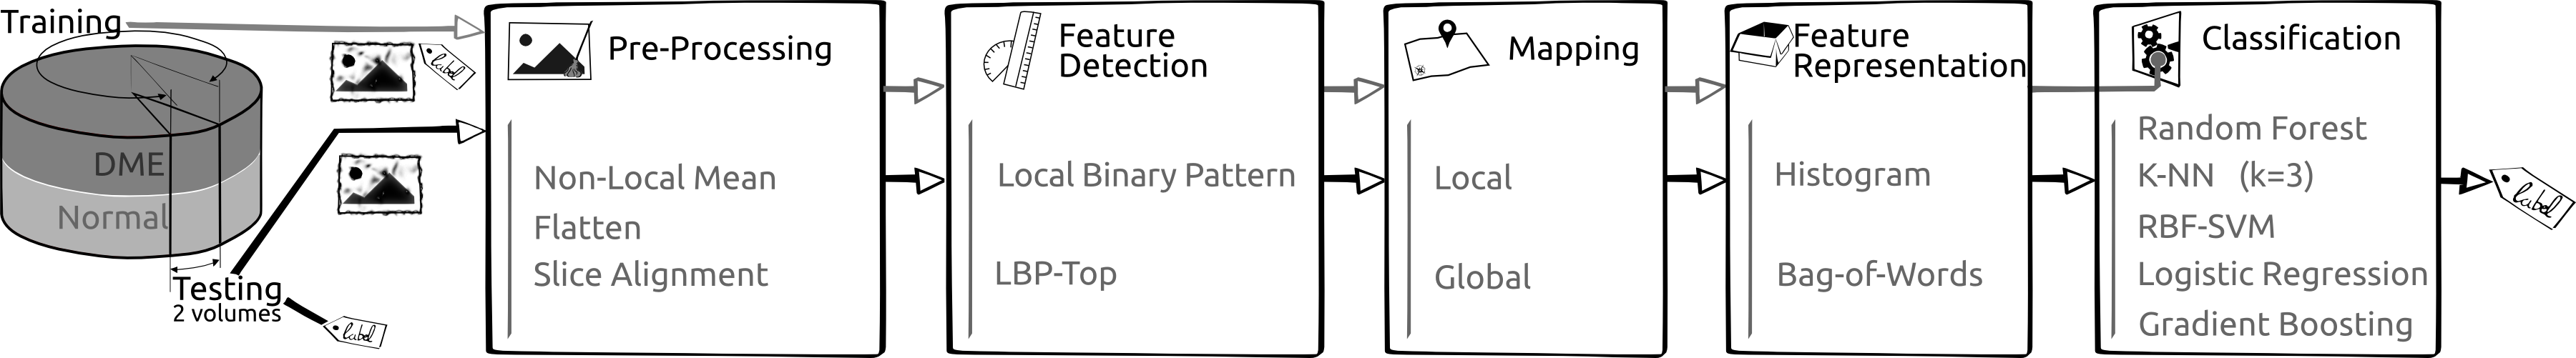
\includegraphics[width=1\linewidth]{ml}}
    \caption{Our proposed classification pipeline.}
  \label{fig:ML-scheme}
\end{figure}



\end{landscape}

